\section{Singular Value Decomposition (SVD)}
Singular Value Decomposition for ad-hoc query support in time-series databases was proposed by Korn et. al. in \cite{citeulike:4373332}. They start with a case study of a typical warehouse dataset (AT\&T) of sale patterns and represent this data as a matrix $X$ of size $N \times M$ with rows corresponding to distinct customers and columns to the time intervals. One of the observations is that the amount of customers is much larger than the length of the time-series: $N>>M$. Another observation is that the size of such a matrix could easily become unmanageable if one must process ``random access'' queries. The proposed solution for this problem is to design a ``compression'' algorithm which trades off some of the precision in order to allow processing of significant amounts of data with random access queries. 

While being aware of some convenient compression techniques such as LZ and Huffman, as well as the spectral decomposition (DFT, DCT and DWT) and clustering techniques, Korn et. al. are arguing that their approach with Singular Value Decomposition is the only solution which does not suffer from CPU-time complexity performance boundaries and performs spectral decomposition in an optimal manner.

The SVD decomposition method is based on a theorem stating that the real-valued matrix $X$ can be expressed as 
\begin{equation}
X = U \times \Lambda \times V^{t}
\label{eq:svd_transform}
\end{equation}
where $U$ is a column-orthonormal $N \times r$ matrix ($r$ is rank of the matrix $X$), $\Lambda$ is a diagonal $r \times r$ matrix of eigenvalues $\lambda_{i}$ of $X$ and $V$ is a column-orthonormal $M \times r$ matrix. Which essentially is the spectral decomposition:
\begin{equation}
X = \lambda_{1} u_{1} \times v_{1}^{t} + \lambda_{2} u_{2} \times v_{2}^{t} + \ldots + \lambda_{r} u_{r} \times v_{r}^{t}
\label{eq:svd_spectrum}
\end{equation}
of the matrix $X$ where $u_{i}$ and $v_{i}$ are column vectors of the $U$ and $V$ and $\lambda_{i}$ is a diagonal elements of $\Lambda$.

Once $X$ is decomposed (two passes over the matrix) into the form of spectrum \ref{eq:svd_spectrum}, the authors suggest to truncate the sum in equation to the first $k$ terms, $k \leq r \leq M$:
\begin{equation}
\hat{X} = \sum_{i=1}^{k} \lambda_{i} u_{i} \times v_{i}
\label{eq:svd}
\end{equation}
where $k$ depends on the space restriction. Note, that these $k$ terms also known as the ``principal components'' in the PCA analysis \cite{citeulike:167581}. 

It is shown that the compression ratio after applying the SVD transform is 
\begin{equation}
s = \frac{N*k + k + k + k*M}{N*M} \approx \frac{k}{M}
\label{eq:svd_compression}
\end{equation}
since $N >> M \geq k$. and the reconstruction of the any cell of the original matrix $\hat{X}$ takes only $O(k)$ time:
\begin{equation}
\hat{x}_{i,j}  = \sum_{m=1}^{k} \lambda_{m} * u_{i,m} * v_{j,m},\; i=1,...,N;\; j=1,...,M
\label{eq:svd_reconstruct}
\end{equation}

Since the SVD approximation could yield considerable errors when restoring some of the original data, authors suggest keeping correcting information in the form of tuples $(row,column,delta)$ for the values which approximate poorly (outliers), calling this method as ``SVD with Details'' or SVDD. 

\begin{figure}[tbp]
   \centering
   \includegraphics[height=55mm]{svd.eps}
   %%{seriesheatmap}
   \caption{The Reconstruction Error (RMSPE) versus disk storage space (\%) for clustering, DCT, SVD and SVDD.}
   \label{fig:svd_benchmark}
\end{figure} 

With respect to the performance of both SVD and SVDD methods, they were compared with DCT (Discrete Cosine Transform, which was shown to be more efficient than DFT \cite{citeulike:4303331}, \cite{citeulike:4501572}) and the S-PLUS embedded clustering method and found to be significantly superior (Figure  \ref{fig:svd_benchmark}), especially SVDD, with the growth of the space allowed to use for corrective information storage.